% !TEX root = ../report.tex
\section{Die Benutzeroberfläche}
\begin{Spacing}{\mylinespace}

Nachdem die Grundfunktionalität der Hauptkomponenten unseres Systems standen ging es nun daran eine einfache aber dennoch funktionale Benutzeroberfläche zu entwerfen. Da das \textit{XNA-Framework} von Haus aus auf \textit{Windows-Forms} zur Darstellung von Benutzeroberflächen setzt, beschlossen auch wir vorerst diese Variante zu nutzen. Hielten uns aber die Möglichkeit offen eventuell später auf das etwas modernere \textit{WPF}-System zu wechseln.
\\\\
Hauptanforderungen waren ein übersichtliches Design und ein einfaches Hinzufügen von neuen Funktionalitäten. Um diese Anforderungen zu erfüllen entschieden wir uns für eine schlichte Statusleiste am unteren Rand des Editor-Fensters für einfache Anzeigen wie zum Beispiel die Frames Pro Sekunde(FPS) oder die Anzahl der Partikel und ein Tab-Panel an der rechten Seite des Editor-Fensters zur Konfiguration der einzelnen Komponenten. Durch die Nutzung des Tab-Panel lässt sich eine gute Separierung der einzelnen Komponenten in der Benutzeroberfläche realisieren. 
\\\\
Die Kommunikation zwischen der Benutzeroberfläche und den einzelnen Komponenten ist über das im \textit{.Net-Framework} integrierte Event-System realisiert. Bei einer Interaktion mit der Benutzeroberfläche wird ein entsprechendes Event gefeuert, welches die benötigten Daten an alle Komponenten liefert, die sich zuvor für dieses Event registriert haben.  

\begin{figure}[h!]
	\vspace*{30px}
	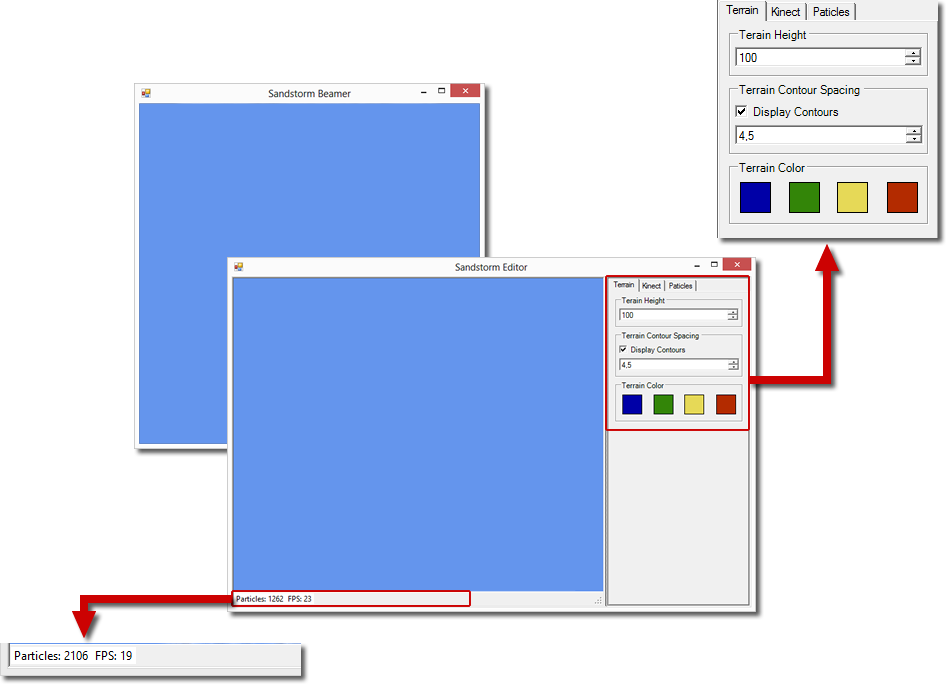
\includegraphics[width=\columnwidth]{graphics/gui.png}	
	\caption{Die GUI}
	\label{fig:GUI}
\end{figure}

\end{Spacing}
\newpage
\clearpage
%% End Of Doc